\documentclass[11pt, oneside]{article} 	% use "amsart" instead of "article" for AMSLaTeX format
\usepackage{geometry} 		% See geometry.pdf to learn the layout options. There are lots.
\geometry{letterpaper}  		% ... or a4paper or a5paper or ... 
\usepackage[parfill]{parskip} 		% Activate to begin paragraphs with an empty line rather than an indent
\usepackage{graphicx}				% Use pdf, png, jpg, or eps§ with pdflatex; use eps in DVI mode
								% TeX will automatically convert eps --> pdf in pdflatex		
\usepackage{amssymb}
\usepackage{amsmath}
\usepackage{authblk}
\usepackage[
backend=biber,
style=alphabetic,
]{biblatex}
\usepackage{graphicx}
\graphicspath{ {./images/} }
\usepackage{verbatim}
\usepackage{tikz} 
\usepackage{subcaption}
\captionsetup{compatibility=false}



\usepackage{syntonly}

% \syntaxonly \langle -- use this for checking syntax only
% \mbox {text} - keep together
% \fbox {text} - keep together and draw around

%\pagestyle{plain|headings|empty} % header and footer p.27
%SetFonts
%\include{filename}, \includeonly{filename1, filename2} , \input[fiename}

%SetFonts% 


\title{Dinosaur War: A Strategic Game of Utter Chance}
\author{Dave Fetterman}
\affil{Obviously Unemployed}
\date{3/2/23}
\begin{document}
\maketitle

\begin{abstract}

We present a modified version of the simple game \emph{War} with an equal deck set, no replacement, and dealer choice, invented in large part and played by my preschool children.  Unlike  \emph{War}, there are choices that must be made by the players.  But like  \emph{War}, the outcome of the game, when played by rational agents, remains 100 percent chance.  This new game, \emph{Dinosaur War}, resembles something more akin to \emph{Rock-Scissors-Paper}; knowing an opponent's guess can guarantee a win, but like  \emph{Rock-Scissors-Paper}, we show a Nash Equilibirum occurs if both players randomize their guesses uniformly across their options.  This result is intuitive but non-obvious.

Therefore:
\begin{itemize}
\item You can play optimally against your child by paying no attention at all.
\item Expect a Pokemon-branded version to hit the shelves soon.
\end{itemize}

\end{abstract}

\section{The Game}


\begin{figure}
\centering
\includegraphics[scale=.3]{cards}
\caption{Dinosaur Cards}
\end{figure}

Children's games need to be simple. The game \emph{Memory} has seen innumerable rebranded recreations, not least because the mechanic is approachable (and nominally educational) but because it can be sold repeatedly, with cartoon characters, animals, or whatever to engage a short attention span.  A set of\emph{Memory} comes with matched pairs of cards with identical backs.  Once the main mechanic is exhausted, the enterprising child will find some other game to create with them.  Here is that game, \emph{Dinosaur War}, created with the cards like those in Figure 1.

\subsection{Rules of Dinosaur War}

\begin{itemize} 
\item Players establish a ranking of cards.  Those might be the commonly-accepted Ace-to-2 of a deck of playing cards, or ``Baryonyx beats Mosasaurus beats T-Rex... beats Apatosaurus'' in Figure 1.
\item Two players get each get an identical deck of these cards.  They were unique in this set but need not be.  Players conceal their hand (though the content of the hands is well-known to those tracking it).
\item At each turn:
\begin{itemize}
\item Each player simultaneously plays a card face up.
\item The player whose card outranks the others gets one point. If there is a tie, no points are awarded. The two played cards are set aside.
\item Play continues until the cards are exhausted.
\end{itemize}
\item The player with the most points at the end wins.
\end{itemize}

The maximum score individual score is 9 (since your opponent's 10 cannot be beat, only tied).  Ties are relatively common.  

\subsection{``Strategy'' in Dinosaur War}

Intuitively, your hand has a certain amount of ``power'' that you deploy to beat an opponent; spending the minimum amount of ``power'' to win preserves better cards for later.  

Imagine on the first turn of a 10 card deck $\{1, 2, ... 10\}$, players $(P_1, P_2)$ play respective cards $(9, 10)$.  This means:
\begin{itemize}
\item $P_2$ takes a one-point lead.
\item 10 is preserved for $P_1$.  They will necessarily win one hand in the future.
\item The powerful card 9 is lost for $P_1$.
\end{itemize}

Alternatively, imagine the first move is $(1,10)$.  This means:

\begin{itemize}
\item $P_2$ takes a one-point lead.
\item 10 is preserved for $P_1$.  They will necessarily win one hand in the future.
\item 1 is lost for $P_1$, the worst card in the hand.
\item Each card of $P_1$'s hand beats at least one card in $P_2$'s hand.
\end{itemize}

The second scenario \emph{seems} better \footnote{In this paper, we measure goodness by expected tricks taken by the hand.}.  But how much better?  And how can one strategically strive to lose bad cards and win ``by just enough'' to take tricks?  This is the focus of the paper.

\subsection{A reduced example}

\begin{figure}
\centering
\begin{subfigure}{.5\textwidth}
  \centering
$ \left[\begin{array}{ccc}
                        & \mathbf{1} & \mathbf{3}\\ 
                       \mathbf{1} & 0 & 0\\
                        \mathbf{3} & 0 & 0\\
                      \end{array}\right] 
$
  \caption{Even 2x2 game}
\label{fig:even_2x2}
\end{subfigure}

\begin{subfigure}{.5\textwidth}
  \centering
$ \left[\begin{array}{ccc}
                        & \mathbf{3} & \mathbf{4}\\ 
                       \mathbf{1} & 0 & 0\\
                        \mathbf{5} & 0 & 0\\
                      \end{array}\right] 
$
  \caption{Another even 2x2 game}
\label{fig:another_even_2x2}
\end{subfigure}

\begin{subfigure}{.5\textwidth}
  \centering
$ \left[\begin{array}{ccc}
                        & \mathbf{1} & \mathbf{3}\\ 
                       \mathbf{2} & 2 & 0\\
                        \mathbf{4} & 0 & 2\\
                      \end{array}\right] 
$
  \caption{Uneven 2x2 game}
\label{fig:uneven_2x2}
\end{subfigure}
\caption{Simple 2x2 games}
\label{fig:2x2}
\end{figure}

Throughout, we'll use the following conventions:
\begin{itemize}
\item $P_1$'s available options are listed in bold down the left column of the payoff matrix (Fig 2a, 2b).
\item $P_2$'s available options are listed in bold across the top row.
\item A trick has a payoff of $1$ if $P_1$ wins, and $-1$ if $P_2$ wins.  $P_1$ is trying to get the total score as high above zero as possible, $P_2$ below.
\item For these payoff matrices $M$, the cell at row $i$, column $j$ is the value of that trick, plus the expected value of the remaining game.
\end{itemize}

This is easy to see in Fig 2a, where the hands are identical.  There are only four games of $(P_1, P_2)$ move pairs:
\begin{itemize}
\item $(1,1)$ means the first trick payoff is zero, and the rest of the game (necessarily $(3,3)$) is determined, also of payoff zero.
\item $(3,3)$ follows similarly.
\item $(3,1)$ means the first trick payoff is 1, and the rest of the game (necessarily $(1,3)$) pays off -1, for a total of zero.
\item $(1,3)$ follows in reverse, with another time game.
\end{itemize}

It's clear that \emph{any strategy} is equivalent in this very boring small game.  \emph{$P_1$ could even announce his moves before $P_2$ selects a card, and the result of the game is still determined.}  The expected value of the game is zero.

Observe in figure 2b that starting sets of $P_1: \{1,5\}, P_2: \{3,4\}$, while not identical, also yield this result; the choices don't matter in the end.

But some uneven sets of cards, like in Fig 2c, are different.
\begin{itemize}
\item If $P_1$ is able to play his 2 against a 1 (on either first or second trick), he wins both tricks for a score of 2.
\item If $P_1$ plays his 2 against a 3, this trick score is -1, but guaranteed to balance by the imminent (or recently played) $(4,1)$ trick, for a total of zero.
\end{itemize}

This is more like \emph{Rock-Scissors-Paper}: knowing your opponent's choice wins you the game.  However, like RSP, the existence of better choices does not mean that there exists a perfect-information strategy that benefits one player.

How can we quantify the goodness of one hand versus another?  We introduce a metric for this particular game \footnote{which should not be conflated with a \emph{dominant} Nash strategy} called the \emph{Dominance Score} and use this to compute the expected value of more complicated (larger) games.

\section{Dominance Score}
\begin{itemize}
\item For each pair
\item Draw the bipartite graph for [2,3,4] vs. [1,2,3]
\end{itemize}

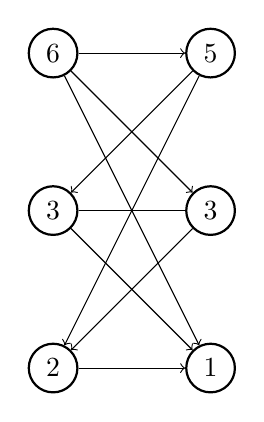
\begin{tikzpicture}
\begin{scope}[every node/.style={circle,thick,draw}]
    \node (1) at (0,0) {2};
    \node (2) at (0,2) {3};
    \node (3) at (0,4) {6};
    \node (4) at (2,0) {1};
    \node (5) at (2,2) {3};
    \node (6) at (2,4) {5};
\end{scope}

\draw[->] (1) -- (4); 
\draw[<-] (1) -- (5); 
\draw[<-] (1) -- (6); 
\draw[->] (2) -- (4); 
\draw[-] (2) -- (5); 
\draw[<-] (2) -- (6); 
\draw[->] (3) -- (4); 
\draw[->] (3) -- (5); 
\draw[->] (3) -- (6); 

\end{tikzpicture}

\section{Dominance in Dino Matrices}

\begin{itemize}
\item 1. The payout matrix always sums to the graph's domination score on every row and column
\item for first row play $V_1$, all $(V_[2,n], H_[1,n])$ pairs are represented n-1 times, all with a weight of /(n-1), by inductive hypothesis
\item This is $(n-1)$ times the domination score of the bipartite graph without $V_1$.
\item the first row $(V_1, H_[1,n])$ repped once.
\item therefore, the complete bipartite graph is repped exactly once in weight.
\end{itemize}

$ \left[\begin{array}{cc}
                        &  \mathbf{5}\\ 
                        \mathbf{6} & 1\\
                      \end{array}\right] 
$

$ \left[\begin{array}{ccc}
                        & \mathbf{3} & \mathbf{5}\\ 
                       \mathbf{3} & 1 & 0\\
                        \mathbf{6} & 0 & 1\\
                      \end{array}\right] 
$

\begin{figure}
\centering
\begin{subfigure}{.5\textwidth}
  \centering
  
\[
\left[ 
\begin{array}{c@{}c@{}c@{}c}
& \mathbf{1} & \mathbf{3} & \mathbf{5} \\


\mathbf{2} &  \left[\begin{array}{ccc}
                        & \mathbf{3} & \mathbf{5}\\ 
                       \mathbf{3} & 1 & 0\\
                        \mathbf{6} & 0 & 1\\
                      \end{array}\right] 
                      & \left[\begin{array}{ccc}
                        & \mathbf{1} & \mathbf{5}\\ 
                       \mathbf{3} & 2 & 0 \\
                        \mathbf{6} & 0 & 2 \\
                      \end{array}\right]   
                      & \left[\begin{array}{ccc}
                        & \mathbf{1} & \mathbf{3}\\ 
                       \mathbf{3} & 2 & 1 \\
                        \mathbf{6} & 1 & 2 \\
                      \end{array}\right]   \\                      
                      
  \mathbf{3} & \left[\begin{array}{ccc}
                        & \mathbf{3} & \mathbf{5}\\ 
                        \mathbf{2} &0 & 0 \\
                        \mathbf{6} & 0 & 0 \\
                      \end{array}\right]
                      & \left[\begin{array}{ccc}
                        & \mathbf{1} & \mathbf{5}\\ 
                       \mathbf{2} & 2 & 0 \\
                        \mathbf{6} & 0 & 2 \\
                      \end{array}\right]   
                      & \left[\begin{array}{ccc}
                        & \mathbf{1} & \mathbf{3}\\ 
                       \mathbf{2} & 2 & 0 \\
                        \mathbf{6} & 0 & 2 \\
                      \end{array}\right]   \\                          
                      
                      
\mathbf{6} &  \left[\begin{array}{ccc}
                        & \mathbf{3} & \mathbf{5}\\ 
                       \mathbf{2} & -2 & -1 \\
                        \mathbf{3} & -1 & -2 \\
                      \end{array}\right] 
& \left[\begin{array}{ccc}
                        & \mathbf{1} & \mathbf{5}\\ 
                       \mathbf{2} & 0 & 0 \\
                        \mathbf{3} & 0 & 0 \\
                      \end{array}\right]   
                      & \left[\begin{array}{ccc}
                        & \mathbf{1} & \mathbf{3}\\ 
                       \mathbf{2} & 1 & 0 \\
                        \mathbf{3} & 0 & 1 \\
                      \end{array}\right]   \\    
\end{array}\right]
\]    
  \caption{Recursive game matrix}
\label{fig:236135_recursive}
\end{subfigure}

\begin{subfigure}{.5\textwidth}
\[
\left[ 
\begin{array}{c@{}c@{}c@{}c}
& \mathbf{1} & \mathbf{3} & \mathbf{5} \\


\mathbf{2} &  (\mathit{1} + .5 = 1.5) & (\mathit{-1} + 1 = 0) & (\mathit{-1} + 1.5 = .5) \\
\mathbf{3} &  (\mathit{1} +0 =  1) & (\mathit{0} + 1 = 1) & (\mathit{-1} + 1 = 0) \\                         
 \mathbf{6} & (\mathit{1} + -1.5 = -.5) & (\mathit{1} + 0 = 1) & (\mathit{1} + .5 = 1.5) \\
\end{array}\right]
\]    
\caption{Payoff matrix}
\label{fig:236135_payoff}
\end{subfigure}

\caption{$\{2,3,6\}$ vs. $\{1,3,5\}$}
\label{fig:236135}
\end{figure}




\begin{figure}
\centering
\begin{subfigure}{.5\textwidth}
  \centering
  
\[
\left[ 
\begin{array}{c@{}c@{}c@{}c}
& \mathbf{1} & \mathbf{3} & \mathbf{6} \\
\mathbf{2} &  \left[\begin{array}{ccc}
                        & \mathbf{3} & \mathbf{6}\\ 
                       \mathbf{3} & 0 & 0\\
                        \mathbf{6} & 0 & 0\\
                      \end{array}\right] 
                      & \left[\begin{array}{ccc}
                        & \mathbf{1} & \mathbf{6}\\ 
                       \mathbf{3} & 1 & 0 \\
                        \mathbf{6} & 0 & 1 \\
                      \end{array}\right]   
                      & \left[\begin{array}{ccc}
                        & \mathbf{1} & \mathbf{3}\\ 
                       \mathbf{3} & 2 & 1 \\
                        \mathbf{6} & 1 & 2 \\
                      \end{array}\right]   \\                      
                      
  \mathbf{3} & \left[\begin{array}{ccc}
                        & \mathbf{3} & \mathbf{6}\\ 
                        \mathbf{2} &-1 & 0 \\
                        \mathbf{6} & 0 & -1 \\
                      \end{array}\right]
                      & \left[\begin{array}{ccc}
                        & \mathbf{1} & \mathbf{6}\\ 
                       \mathbf{2} & 1 & 0 \\
                        \mathbf{6} & 0 & 1 \\
                      \end{array}\right]   
                      & \left[\begin{array}{ccc}
                        & \mathbf{1} & \mathbf{3}\\ 
                       \mathbf{2} & 2 & 0 \\
                        \mathbf{6} & 0 & 2 \\
                      \end{array}\right]   \\                          
                      
                      
\mathbf{6} &  \left[\begin{array}{ccc}
                        & \mathbf{3} & \mathbf{6}\\ 
                       \mathbf{2} & -2 & -1 \\
                        \mathbf{3} & -1 & -2 \\
                      \end{array}\right] 
& \left[\begin{array}{ccc}
                        & \mathbf{1} & \mathbf{6}\\ 
                       \mathbf{2} & 0 & 0 \\
                        \mathbf{3} & 0 & 0 \\
                      \end{array}\right]   
                      & \left[\begin{array}{ccc}
                        & \mathbf{1} & \mathbf{3}\\ 
                       \mathbf{2} & 1 & 0 \\
                        \mathbf{3} & 0 & 1 \\
                      \end{array}\right]   \\    
\end{array}\right]
\]    
  \caption{Recursive game matrix}
\label{fig:236136_recursive}
\end{subfigure}

\begin{subfigure}{.5\textwidth}
\[
\left[ 
\begin{array}{c@{}c@{}c@{}c}
& \mathbf{1} & \mathbf{3} & \mathbf{6} \\


\mathbf{2} &  (\mathit{1} + 0 = 1) & (\mathit{-1} + .5 = -.5) & (\mathit{-1} + 1.5 = .5) \\
\mathbf{3} &  (\mathit{1} -.5  =  .5) & (\mathit{0} + .5 = .5) & (\mathit{-1} + 1 = 0) \\                         
 \mathbf{6} & (\mathit{1} -1.5 = -.5) & (\mathit{1} + 0 = 1) & (\mathit{0} + .5 = .5) \\
\end{array}\right]
\]    
\caption{Payoff matrix}
\label{fig:236136_payoff}
\end{subfigure}

\caption{$\{2,3,6\}$ vs. $\{1,3,6\}$}
\label{fig:236136}
\end{figure}


\section{Nash equilibria in an even strategy}
\begin{itemize}
\item 2. On such a matrix, there is a nash equilibrium of all evens, where deviating doesn't improve prospects.
\item presume all weights are even
\item shifting epsilon from one of the rows can't increase your score as row player, if the col player doesn't move.
\item If this changes the weighted sum of a column, then player 2 can improve his EV.
\item If this changes no columns, then the two rows are identical.
\item if it's 123 vs.  789, you can obvously choose whatever probabilities you like.
\end{itemize}

\section{Considerations and Examples}
\begin{itemize}
\item 3. Some theorem - nash equilibria all have the same value on a two-person zero-sum game.
\item Minimax theorem, von Neumann, 1928 TODO    
\item Corollary of Maximin: All nash equilibira have saem value - minimax (or maximin)
\item 4. Therefore, even is an optimal strategy.
\item Note: Not THE optimal strategy.
\item  5. Of course, knowing or guessing the opponent's actual move is an advantage.S
\item Show the table for 10 v 10
\end{itemize}

\section{10 v. 10 payoffs}

TODO: Write the code

\section{Pieceyard}


\begin{thebibliography}{9}
\bibitem{1}
Wikipedia: \url{https://en.wikipedia.org/wiki/Minimax_theorem}
\end{thebibliography}


\end{document}

